\begin{figure}[H]
\centering
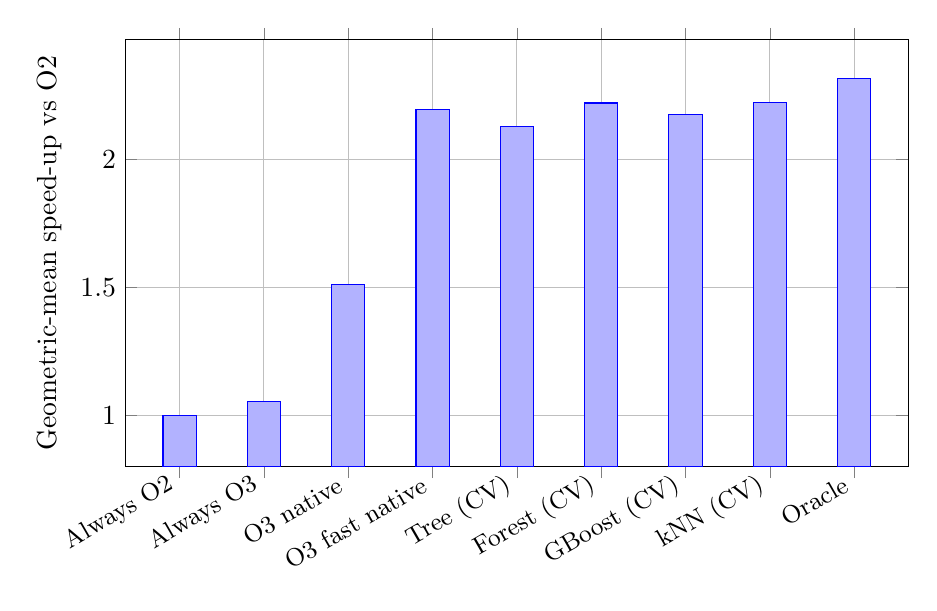
\begin{tikzpicture}
\begin{axis}[
    ybar, width=0.95\textwidth, height=7cm,
    ylabel={Geometric-mean speed-up vs O2},
    symbolic x coords={Always O2,Always O3,O3 native,O3 fast native,Tree (CV),Forest (CV),GBoost (CV),kNN (CV),Oracle},
    xtick=data, x tick label style={rotate=30,anchor=east,font=\small},
    ymin=0.8, 
    bar width=12pt,
    enlarge x limits=0.08,
    legend style={at={(0.5,1.03)},anchor=south,legend columns=-1,font=\small},
    grid=major]
\addplot coordinates {(Always O2,1.0000) (Always O3,1.0539) (O3 native,1.5122) (O3 fast native,2.1971) (Tree (CV),2.1300) (Forest (CV),2.2207) (GBoost (CV),2.1751) (kNN (CV),2.2215) (Oracle,2.3164)};

\end{axis}
\end{tikzpicture}
\caption{Geometric-mean speed-up over \texttt{O2} of the static configurations, the decision models (5-fold CV) and the oracle.}
\label{fig:speedup}
\end{figure}
